%versi 3 (22-07-2020)
\chapter{Landasan Teori}
\label{chap:teori}

% label: {what for}:{page}:{section}:{subsection}:{name}

\section{SharIF Judge}
\label{sec:2:sharifjudge}

SharIF Judge merupakan modifikasi dari \textit{open source} bernama Sharif Judge, sebuah website judge gratis dengan kemampuan mengkompilasi bahasa C, C++, Java, dan Python. Sharif Judge dibuat oleh Mohammad Javad Naderi dengan interface web berbahasa PHP menggunakan \textit{framework} CodeIgniter 3 dan BASH~\cite{sharif}. Modifikasi dilakukan untuk menambahkan fitur pada Sharif Judge dan juga untuk menyesuaikan sesuai dengan kebutuhan Teknik Informatika UNPAR.

\subsection{Instalasi}
\label{sub:2:1:instalasi}

Ada beberapa prasyarat yang diperlukan dalam menjalankan SharIF Judge pada sebuah \textit{server} Linux adalah sebagai berikut:

\begin{itemize}
	\item \textit{Webserver} dengan PHP versi 5.3 atau lebih dengan \texttt{mysqli} extension
	\item PHP Command Line Interface (CLI)
	\item \textit{Database} MySql atau PostgreSql
	\item PHP harus memiliki akses untuk menjalankan \textit{shell commands} dengan fungsi \verb|shell_exec|
	\item Kemampuan untuk mengompilasi dan menjalankan kode yang dikumpulkan (\texttt{gcc}, \texttt{g++}, \texttt{javac}, \texttt{java}, \texttt{python2}, dan \texttt{python3})
	\item Perl
\end{itemize}

Setelah perangkat yang sudah memenuhi prasyarat, berikut merupakan cara instalasi SharIF Judge:

\begin{enumerate}
	\item Unduh versi terakhir dari Sharif Judge dan menempatkannya pada direktori publik.
	\item Pindahkan folder \texttt{system} dan \texttt{application} ke luar direktori publik. Kemudian simpan alamatnya pada \texttt{index.php}.
	\item Buat sebuah \textit{Database} MySql atau PostgreSql.
	\item Atur pengaturan koneksi \textit{database} pada \texttt{application/config/database.php}.
	\item Atur pengaturan koneksi \texttt{RADIUS} dan \texttt{SMTP} pada \texttt{application/config/secrets.php} jika dibutuhkan.
	\item Atur agar direktori \texttt{application/cache/Twig} dapat ditulis oleh php.
	\item Buka halaman utama SharIF Judge pada \textit{browser} dan ikuti proses instalasi.
	\item Log in dengan akun admin
	\item Pindahkan folder \texttt{tester} dan \texttt{assignments} ke luar direktori publik. Kemudian simpan alamatnya pada halaman pengaturan.
\end{enumerate}

\newpage

\subsection{Users}
\label{sub:2:1:users}

Pada SharIF Judge, pengguna dibagi menjadi 4 buah \textit{role}. Role yang tersedia adalah sebagai berikut:

\begin{enumerate}
	\item \textit{admin}
	\item \textit{head instructor}
	\item \textit{instructor}
	\item \textit{student}
\end{enumerate}

Setiap \textit{role} memiliki akses pada aksi yang berbeda berdasakan \textit{role}-nya. Tabel \ref{tab:2:1:fitur_user} merupakan aksi-aksi yang dapat dilakukan untuk setiap pengguna pada SharIF Judge.

\begin{table}[H]
	\centering
	\caption{\textit{Tabel fitur untuk setiap role}}
	\label{tab:2:1:fitur_user}
	\begin{tabular}{|l|c|c|c|c|}
		\hline
		Aksi                              & \textit{Admin} & \textit{Head Instructor} & \textit{Instructor} & \textit{Student} \\

		\hline
		Mengubah \textit{Settings}        & \ding{51}      & \ding{53}                & \ding{53}           & \ding{53}        \\
		Mengelola Pengguna                & \ding{51}      & \ding{53}                & \ding{53}           & \ding{53}        \\
		Mengelola \textit{Assignment}     & \ding{51}      & \ding{51}                & \ding{53}           & \ding{53}        \\

		Mengelola Notifikasi              & \ding{51}      & \ding{51}                & \ding{53}           & \ding{53}        \\
		\textit{Rejudge}                  & \ding{51}      & \ding{51}                & \ding{53}           & \ding{53}        \\
		Mengelola \textit{Queue}          & \ding{51}      & \ding{51}                & \ding{53}           & \ding{53}        \\
		Mendeteksi Kode yang Mirip        & \ding{51}      & \ding{51}                & \ding{53}           & \ding{53}        \\
		Melihat Semua \textit{Submission} & \ding{51}      & \ding{51}                & \ding{51}           & \ding{53}        \\

		Mengunduh Kode Final              & \ding{51}      & \ding{51}                & \ding{51}           & \ding{53}        \\
		Memilih \textit{Assignment}       & \ding{51}      & \ding{51}                & \ding{51}           & \ding{51}        \\
		\textit{Submit} Kode              & \ding{51}      & \ding{51}                & \ding{51}           & \ding{51}        \\

		\hline
	\end{tabular}
\end{table}

\section{CodeIgniter 3}
\label{sec:2:codeigniter}

CodeIgniter 3 adalah sebuah \textit{framework opensource} untuk mempermudah pengguna dalam membangun sebuah aplikasi \textit{website} menggunakan bahasa PHP. CodeIgniter 3 bertujuan untuk membantu pengguna dalam membangun sebuah aplikasi \textit{website} lebih cepat dengan menyedikan \textit{library} yang beragam dengan fungsi yang umum digunakan dan tampilan dan \textit{logic} yang simpel. Gambar \ref{fig:2:ciflowchart} merupakan bagaimana data mengalir pada sistem CodeIgniter.

\begin{figure}[H]
	\centering
	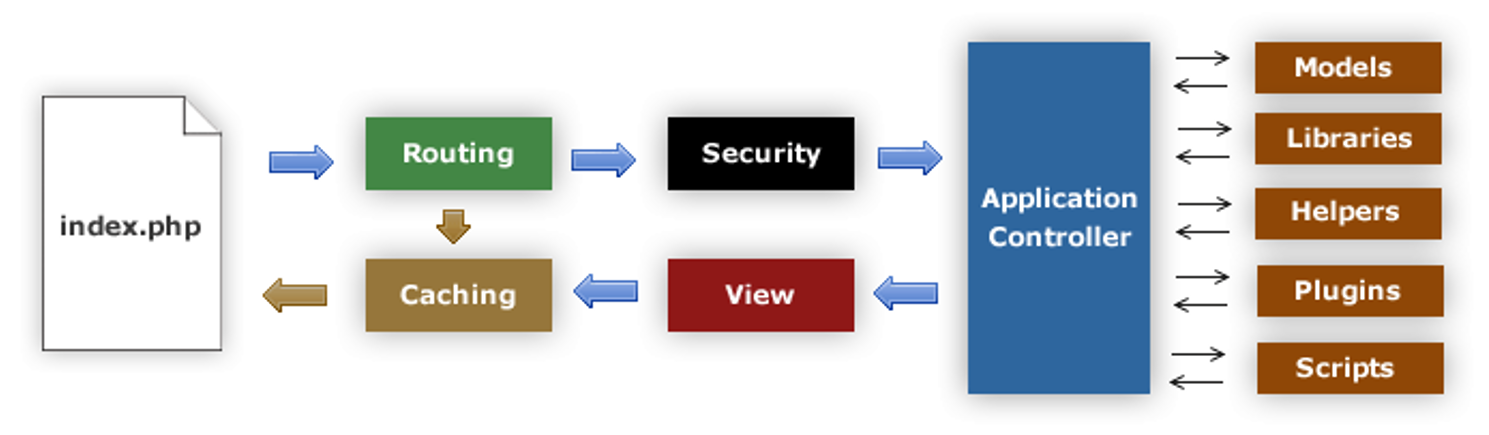
\includegraphics[scale=0.3]{ci-flowchart.png}
	\caption{\textit{Flow Chart} CodeIgniter}
	\label{fig:2:ciflowchart}
\end{figure}

Berikut merupakan penjelasan sederhana dari \textit{flow chart} sistem CodeIgniter 3:

\begin{enumerate}
	\item \verb|index.php| berfungsi sebagai \textit{front controller} yang akan melakukan inisiasi \textit{resource} utama untuk menjalankan CodeIgniter.
	\item Router meneliti \textit{request} HTTP dan menentukan apa yang harus dilakukan dengan \textit{request} tersebut.
	\item Jika terdapat \textit{file cache}, maka langsung dikirimkan ke \textit{browser} melewati eksekusi sistem yang biasanya.
	\item Sebelum \textit{controller} dimuat, seluruh \textit{request} HTTP dan data dari user disaring terlebih dahulu untuk keamanan.
	\item \textit{Controller} memuat \textit{model}, \textit{library} utama, dan \textit{resource} lainnya yang diperlukan.
	\item \textit{View} akhir lalu dikirim ke browser untuk dilihat. \textit{Cache} akan dibuat terlebih dahulu bila diaktifkan.
\end{enumerate}

\subsection{Model-View-Controller}
\label{sub:2:2:modelviewcontroller}

CodeIgniter merupakan framework berbasis arsitektur Model-View-Controller atau yang selanjutnya akan disebut dengan MVC. MVC adalah pendekatan \textit{software} yang memisahkan \textit{logic} aplikasi dan tampilannya. Pendekatan ini membuat \textit{website} hanya memiliki sedikit \textit{script} karena tampilan \textit{website} terpisah dari \textit{scripting} PHP. Berikut merupakan penjelasan mengenai struktur MVC:

\subsubsection{Model}
\label{sub:2:2:1:model}

\textit{Model} mewakili struktur data pada sistem untuk mengambil, memasukkan, dan memperbaharui data pada \textit{database}. \textit{Model} dapat dibuat dengan membuat sebuah kelas yang mengekstensi \verb|CI_Model| dan diletakkan pada \verb|application/models/|.

% TODO: Masukkin ke dlm folder kode
\begin{lstlisting}[language=php, caption=Contoh \textit{model}, label=kode:2:2:1:model]
class Blog_model extends CI_Model {

	public $title;
	public $content;
	public $date;

	public function get_last_ten_entries()
	{
			$query = $this->db->get('entries', 10);
			return $query->result();
	}

	public function insert_entry()
	{
			$this->title    = $_POST['title'];
			$this->content  = $_POST['content'];
			$this->date     = time();

			$this->db->insert('entries', $this);
	}

	public function update_entry()
	{
			$this->title    = $_POST['title'];
			$this->content  = $_POST['content'];
			$this->date     = time();

			$this->db->update('entries', $this, array('id' => $_POST['id']));
	}

}
\end{lstlisting}

Kode \ref{kode:2:2:1:model} merupakan contoh model kelas bernama \verb|Blog_model| pada CodeIgniter. \textit{Model} \verb|Blog_model| dapat mengambil, menambahkan, dan memperbaharui \textit{database} bernama `entries'. File \textit{model} tersebut akan disimpan pada \verb|application/models/Blog_model|. Selanjutnya, pengguna dapat memanggil \textit{Model} tersebut pada \textit{file controller} (akan dijelaskan pada bagian \hyperref[sub:2:2:3:Controller]{Controller}) untuk memanggil model pada Kode \ref{kode:2:2:1:model} dengan mengunakan notasi sebagai berikut:

\begin{center}
	\verb|$this->load->model('Blog_model');|.
\end{center}

Untuk memanggil \textit{method} yang terdapat pada model tersebut, notasi yang digunakan adalah sebagai berikut:

\begin{center}
	\verb|$this->Blog_model->get_last_ten_entries();|
\end{center}

Notasi diatas akan memuat \verb|model| dengan nama \verb|Blog_model| dan akan memanggil \textit{method} \verb|get_last_ten_entries|.

\subsubsection{View}
\label{sub:2:2:2:View}

\textit{View} adalah informasi yang akan di tunjukkan kepada user. Biasanya \textit{view} merupakan sebuah halaman web, tetapi pada CodeIgniter, view dapat berupa pecahan halaman seperti \textit{header, footer, sidebar}, dan lainnya. Pecahan halaman tersebut dapat dimasukkan secara fleksibel ke dalam \textit{view} lainnya apabila dibutuhkan.

\begin{lstlisting}[language=php, caption={Contoh \textit{view}}, label={kode:2:2:2:view}]
<html>
<head>
        <title>My Blog</title>
</head>
<body>
        <h1>Welcome to my Blog!</h1>
</body>
</html>
\end{lstlisting}

Kode \ref{kode:2:2:2:view} merupakan contoh dari \textit{file view} pada CodeIgniter. File akan disimpan pada direktori \verb|application/views/|. Untuk dapat diperlihatkan dibutuhkannya penggalian halaman pada \textit{file controller} dengan cara sebagai berikut:

\begin{center}
	\verb|$this->load->view(`name');|
\end{center}

Notasi diatas akan mengembalikan halaman \textit{view} dengan nama \verb|name| yang terletak pada direktori \verb|application/views/name.php| dan menampilkannya kepada pengguna.

\subsubsection{Controller}
\label{sub:2:2:3:Controller}

\textit{Controller} adalah bagian utama dari aplikasi CodeIgniter, berfungsi sebagai perantara antara \textit{model}, \textit{view}, dan \textit{resources} lainnya yang dibutuhkan untuk memproses HTTP \textit{request} dan membuat sebuah web page. Kelas \textit{Controller} akan mengekstensi \verb|CI_Controller| dan disimpan pada \verb|application/controllers/|. Contoh \textit{controller} ditunjukkan pada Kode \ref{kode:2:2:3:controller}.

\begin{lstlisting}[language=php, caption={Contoh \textit{controller}}, label={kode:2:2:3:controller}]
<?php
class Blog extends CI_Controller {

		public function index()
		{
				echo 'Hello World!';
		}

		public function comments()
		{
				echo 'Look at this!';
		}
}
\end{lstlisting}

Kode \ref{kode:2:2:3:controller} berfungsi dalam mengembalikan string sesuai dengan fungsi \textit{controller} yang dipanggil. Nama file \textit{controller} pada direktori \verb|application/controllers/blog.php| dan metode diatas akan dijadikan segmen pada URL seperti berikut:

\begin{center}
	\verb|example.com/index.php/blog/index/|
\end{center}

URL diatas akan mengembalikan sebuah teks `Hello World!'.

\begin{lstlisting}[language=php, caption=Contoh memuat \textit{model} dan menampilkan \textit{view}, label=kode:2:2:3:cimodelview]
class Blog_controller extends CI_Controller {
		public function blog()
		{
				$this->load->model('blog');

				$data['query'] = $this->blog->get_last_ten_entries();

				$this->load->view('blog', $data);
		}
}
\end{lstlisting}

Pada CodeIgniter, \textit{model} dan \textit{view} hanya dapat dimuat melalui controller. Seperti contoh, Kode \ref{kode:2:2:3:cimodelview} akan memuat \textit{model} \verb|blog| dan mengambil data dari \textit{database}, lalu menampilkan \textit{view} yang memuat data tersebut.

\subsection{CodeIgniter URLs}
\label{sub:2:2:codeigniterurls}

URL pada CodeIgniter menggunakan \textit{segment-based approach} dibandingkan dengan \textit{query string approach} yang biasanya dipakai. \textit{Segment-based approach} dirancang untuk \textit{search-engine} dan dapat mempermudah pengguna juga. Berikut merupakan contoh dari URL CodeIgniter:

\begin{center}
	\verb|example.com/news/article/my_article|
\end{center}

Struktur URL pada CodeIgniter juga mengikuti pendekatan MVC (referensi \ref{sub:2:2:modelviewcontroller}) dan biasanya memiliki struktur sebagai berikut:

\begin{center}
	\verb|example.com/class/function/ID|
\end{center}

\begin{enumerate}
	\item Segmen pertama mewakili kelas \textit{controller} yang ingin dipanggil.
	\item Segmen berikutnya mewakili fungsi kelas atau \textit{method} yang ingin di panggil.
	\item Segmen ketiga dan selanjutnya mewakili \textit{identifier} atau pengenal dan variable-variable lain yang akan di kirimkan ke \textit{controller}.
\end{enumerate}

\section{Twig}
\label{sec:2:twig}

Twig merupakan sebuah \textit{template engine} untuk PHP. Ada beberapa \textit{expression}, \textit{expression}, atau \textit{statement} yang ditemupakan pada template Twig adalah sebagai berikut:
\begin{itemize}
	\item Pewarisan \textit{Template}
	\item Struktur Kontrol (mengunaan kondisional, \textit{looping})
	\item Filter
	\item Variable pada PHP
\end{itemize}

Pada saat template dievaluasi, semua \textit{variable} atau \textit{expression} akan dibuah menjadi value dan \textit{tag} yang mengontrol logika template.

\begin{lstlisting}[language={php}, caption={Contoh template Twig}, label={kode:2:twig}]


	<ul id="navigation">
	
		<li>
			<a href="{{item.href}}">
				&nbsp;&nbsp;
				{{ item.caption|upper }}
			</a>
		</li>
	
	</ul>

\end{lstlisting}

Kode \ref{kode:2:twig} merupakan contoh sebuah template Twig. Terdapat dua jenis \textit{delimiter}, yaitu \verb|| dan \verb|{{ ... }}|. \textit{Delimiter} \verb|| digunakan untuk Menjalankan sebuah \textit{statement} seperti \textit{for-loops}, sedangkan \textit{delimiter} \verb|{{ ... }}| digunakan untuk mengubah sebuah \textit{variable} atau \textit{expression} menjadi nilai sesungguhnya.

\section{Integrated Development Environment}
\label{sec:2:ide}

Intergrated Development Environment (IDE) merupakan sebuah aplikasi yang menyediakan berbagai peralatan yang diperlukan untuk membantu pengembangan perangkat lunak. Beberapa peralatan umum yang dimiliki oleh sebuah IDE adalah sebagai berikut:

\begin{itemize}
	\item \textit{Editor} \\
	      Editor teks sebagai tempat untuk mengetik kode, dapat dilengkapi dengan berbagai fitur seperti \textit{syntax highlighting} (menampilkan teks dengan warna yang berbeda untuk menginkatkan keterbacaan kode) dan \textit{word completion} (menampilkan prediksi kata yang sedang atau yang akan diketik pengguna).
	\item \textit{Complier} \\
	      Digunakan untuk menterjemahkan kode program yang dibuat pada editor teks ke dalam sebuah program yang dapat dijalankan oleh komputer.
	\item \textit{Execution} \\
	      Menjalankan kode program yang sudah dikompilasi, dengan input jika dibutuhkan, dan mengembalikan hasilnya.
\end{itemize}

\section{Ace}
\label{sec:2:ace}

Ace merupakan sebuah editor kode yang dapat dimasukkan ke dalam sebuah website yang dibuah mengunakan bahasa \textit{Javasciprt}. Ace memiliki kemampuan dari editor pada umumnya. Berikut merupakan beberapa fitur utama yang dimiliki oleh Ace:

\begin{itemize}
	\item \textit{Syntax highlighting} untuk bahasa pemrograman.
	\item Automatic indent dan  outdent.
	\item Kemampuan \textit{cut}, \textit{copy}, dan \textit{paste}.
	\item Kemampuan \textit{drag and drop} teks menggunakan mouse.
	\item Banyak \textit{Cursors} dan \textit{selections}
	\item \textit{Line wrapping}
	\item \textit{Code folding}
\end{itemize}

Beberapa kelas penting yang terdapat pada library Ace adalah sebagai berikut:

\begin{itemize}
	\item \verb|Ace| \\
	      Merupakan kelas utama untuk menyiapkan editor kode Ace pada \textit{browser}
	\item \verb|Editor| \\
	      Entri utama untuk fungsionalitas library Ace. Editor sendiri merepresentasikan editor kode yang dibuat pada web. Pada editor sendiri disediakannya \textit{event listener} yaitu sebagai berikut:

	      \begin{enumerate}
		      \item \verb|mouseup| : Mendengarkan saat melepaskan tombol pada tetikus atau \textit{mouse}.
	      \end{enumerate}

	\item \verb|EditSession| \\
	      Sebuah kelas yang menyimpan semua status dalam editor seperti isi editor, \textit{selection}, dan lain-lain. Kelas ini dinamakan \verb|EditSession|, tetapi untuk mengakses dari editor dinamakan \textit{session}. Pada kelas \textit{session} ada beberapa \textit{event listener} yaitu:

	      \begin{enumerate}
		      \item \verb|change| : Mendengarkan perubahan pada isi editor.
		      \item \verb|changeCursor| : Mendengarkan perubahan pada kursor atau \textit{anchor} dalam editor.
		      \item \verb|changeSelection| : Mendengarkan perubahan pemilihan isi kode dalam editor.
	      \end{enumerate}

	\item \verb|Anchor| \\
	      Menangani posisi \textit{pointer} pada dokumen. Saat teks dimasukkan atau dihapus, posisi \textit{anchor} akan diperbaharui.
	\item \verb|Document| \\
	      Menyimpan teks dokumen.
	\item \verb|Range| \\
	      Kelas ini digunakan di berbagai tempat untuk mengindikasikan suatu wilayah di dalam editor. Kelas ini menyimpan posisi baris awal dan kolom awal, serta baris akhir dan kolom akhir.
	\item \verb|Selection| \\
	      Kelas ini menyimpan posisi yang di pilih oleh pengguna dalam editor.
	\item \verb|Commands| \\
	      Kelas ini digunakan untuk menjalankan perintah pada sebuah editor. Contoh perintah yang sudah ada dalam editor yaitu \textit{insert}, \textit{copy}, \textit{paste}. Pada kelas ini tersedia \textit{event listener} untuk mendengarkan segala \textit{event} yang sudah terjadi bernama \verb|afterExec|.
\end{itemize}

\begin{lstlisting}[language={php}, caption={Contoh kode pengunaan Ace}, label={kode:2:5:ace}]
<!DOCTYPE html>
<html lang="en">
<head>
<title>ACE in Action</title>
<style type="text/css" media="screen">
	#editor { 
		position: absolute;
		top: 0;
		right: 0;
		bottom: 0;
		left: 0;
	}
</style>
</head>
<body>

<div id="editor">function foo(items) {
	var x = "All this is syntax highlighted";
	return x;
}</div>
	
<script src="/ace-builds/src-noconflict/ace.js" type="text/javascript" charset="utf-8"></script>
<script>
	var editor = ace.edit("editor");
	editor.setTheme("ace/theme/monokai");
	editor.session.setMode("ace/mode/javascript");
</script>
</body>
</html>
\end{lstlisting}

Kode \ref{kode:2:5:ace} merupakan cara pengunaan Ace pada sebuah \texttt{div} dengan id \texttt{editor}. Ace juga memiliki beberapa konfigurasi, seperti contoh ini yaitu mengunakan tema \textit{monokai} dan mengunakan \textit{syntax highlighting} untuk bahasa pemrograman JavaScript.